% CMSB 2014 poster - BioPreDyn project
\documentclass[17pt,portrait,a1,usenames,dvipsnames,plainboxedsections]{sciposter}
\usepackage{color}
\usepackage[pdftex]{graphicx}
\usepackage{listings}
\usepackage{multicol}
\usepackage[labelfont=bf,font=it]{caption}

\definecolor{BoxCol}{rgb}{0.8,0.835,0.894}

\lstset{
  basicstyle=\small\ttfamily,
  keywordstyle=\color{ForestGreen},
  commentstyle=\color{Gray},
  stringstyle=\color{Fuchsia},
  captionpos=b
}

\begin{document}

\conference{{\bf CMSB 2014}, 12th Conference on Computational Methods in
Systems Biology, 17-19 November 2014, University of Manchester, UK}
\leftlogo{fp7_logo.pdf}
\rightlogo{biopredyn_logo.pdf}
\title{BioPreDyn software: an implementation of the systems biology model
building cycle}
\author{Bertrand Moreau \& Eric Boix}
\institute{The CoSMo Company, Lyon, France}
\email{bertrand.moreau@thecosmocompany.com}
\maketitle

\begin{abstract}
Many methods and tools deal with specific steps of
the systems biology model building cycle for data-driven computational models
\cite{Kitano2002}: data analysis, model building, parameter estimation,
identifiability analysis, uncertainty quantification, model discrimination, and
optimal experimental design. There is still a need for a software platform
supporting the entire cycle; the BioPreDyn project aims at developing such a
platform. Here, we present an integrative software framework for reading and
executing workflows written using the Simulation Experiment Description Markup
Language (SED-ML). The current version handles workflows combining simulation
runs, flux balance analysis and parameter estimation; its application
programming interface (API) provides additional tools for assessing the quality
of a numerical model.
\end{abstract}

\begin{multicols}{2}

\section{Architecture and implementation}
In the scope of the BioPreDyn project, a {\bf simulation workflow} - or
numerical experiment - is defined as a {\bf sequence of instructions} to be
executed on a numerical model; instructions encoded in the workflow include
{\bf model initialization}, {\bf simulation runs} and {\bf result processing}.
Standard languages encodes different parts of the workflow: the Simulation
Experiment Description Markup Language\cite{Kohn2008} ({\bf SED-ML}) for the
workflow itself, the Systems Biology Markup Language\cite{Hucka2003}
({\bf SBML}) for the model, and the Numerical Markup Language ({\bf NuML}) for
the numerical results.

\begin{figure}
\begin{minipage}[c]{0.5\textwidth}
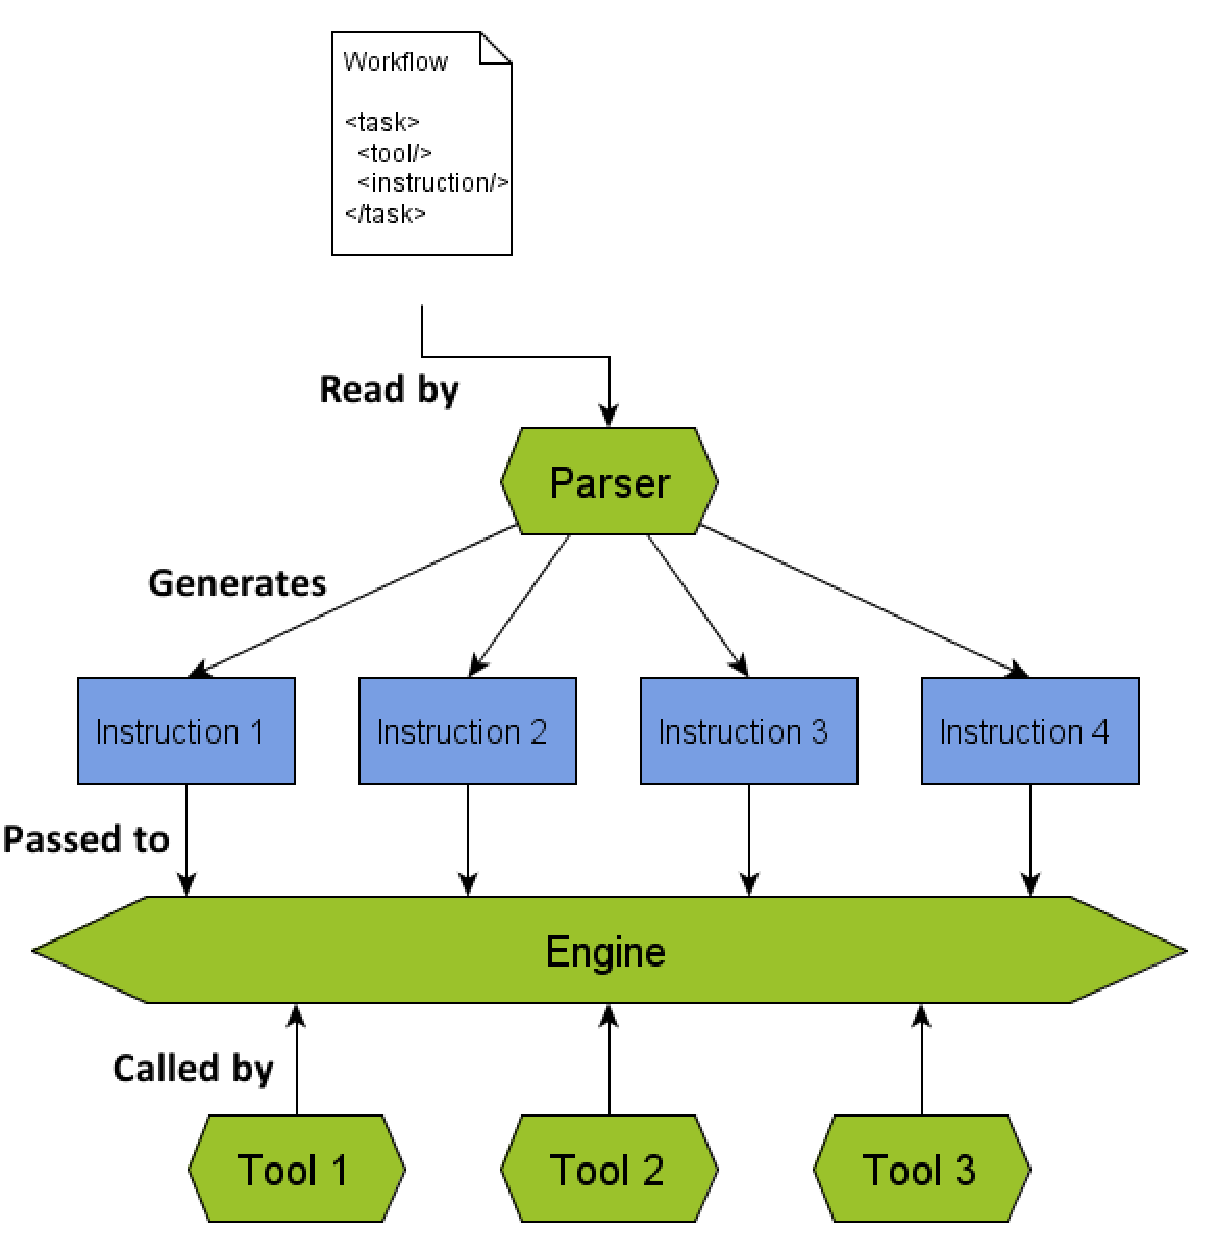
\includegraphics[width=\textwidth]{proposal_complete.pdf}
\end{minipage}\hfill
\begin{minipage}[c]{0.45\textwidth}
\caption{Representation of a simulation workflow in BioPreDyn: a parser reads
the workflow from its physical representation and passes it to the engine as a
series of instructions; each instruction describes an operation and refers to
a model. The engine dispatches the instructions to the appropriate tools and
schedules their execution following the order specified in the input workflow
file. In this context, "executing a workflow" simply means executing each
instruction sequentially.}
\end{minipage}
\end{figure}

An {\bf open-source Python software framework} hosted on the GitHub platform
was developed. The BioPreDyn software relies on several tools for writing or
reading specific file formats, running simulations, accessing data bases, etc:
dedicated parsers, simulation engines, and web services. Depending on the task
to be done, one can therefore choose between {\bf different simulation
engines}.

\begin{figure}
\centering
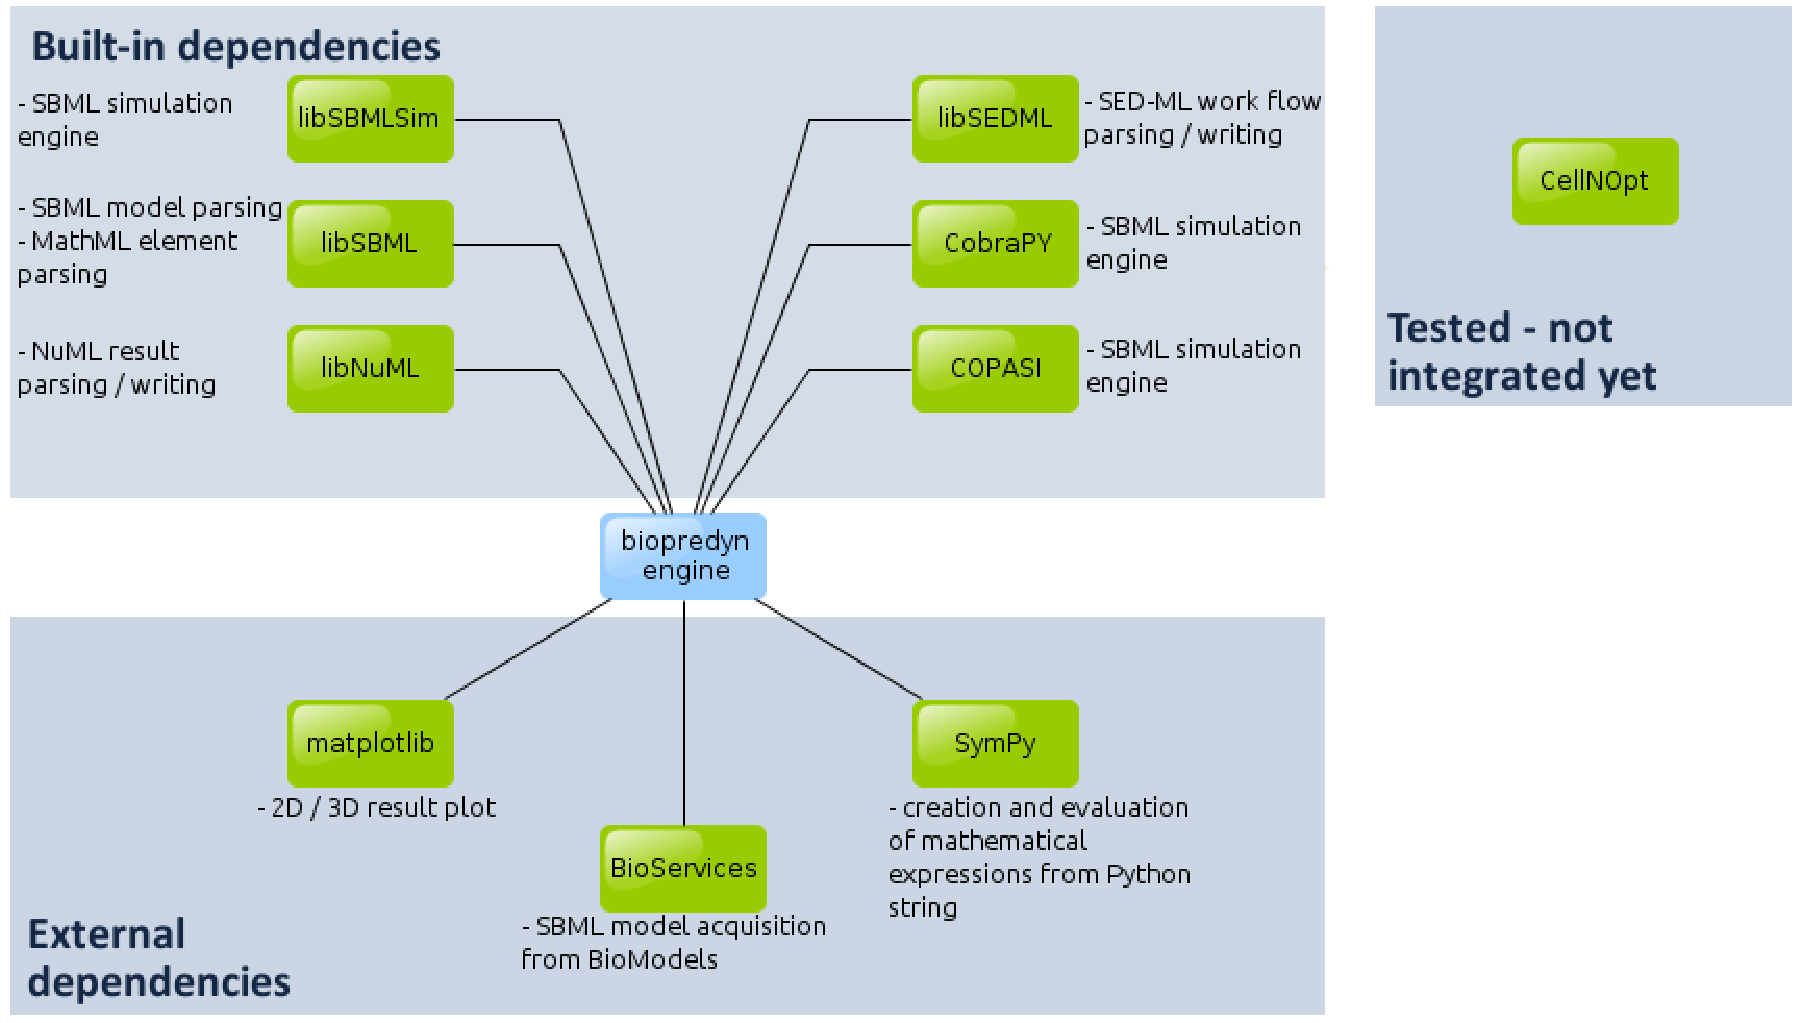
\includegraphics[width=0.95\textwidth]{biopredyn_modules_3.pdf}
\caption{BioPreDyn collection of tools; built-in dependencies are compiled
and wrapped with the package, while external dependencies need to be
installed independently.}
\end{figure}

\section{Usage and results}
The BioPreDyn software's main purpose is to {\bf read and execute SED-ML
encoded workflows}; its default behavior when given a SED-ML file consists in
first running all the tasks, then processing all the outputs, if any. An
elementary executable SED-ML workflow contains at least a {\bf simulation}, a
{\bf model}, and a {\bf task} linking the simulation to the model.
\lstinputlisting[
  language=XML,
  caption={SED-ML workflow describing a time course simulation of an SBML
model hosted on the BioModels database; for the sake of readability, this
workflow does not describe any output nor data generation step.}
]{goldbeter_simulation.xml}
In addition, the BioPreDyn API {\bf can be used as any Python library} to
manipulate and enrich any workflow with operations that are not described by
the SED-ML language yet; one could for instance use the following script to
estimate the parameters of a model:
\lstinputlisting[
  language=Python,
  caption={Example of an executable script using the BioPreDyn API to describe
a parameter estimation based on an SED-ML time course description.}
]{script_example_2.py}
Once a simulation has been run, the biopredyn.result module provides multiple
tools and accessors for {\bf analyzing and exporting results}. Numerical results
can be displayed using Matplotlib\cite{Hunter2007} or exported as CSV of NuML
files.
\begin{figure}
\begin{center}
\begin{minipage}[c]{0.56\textwidth}
\centering
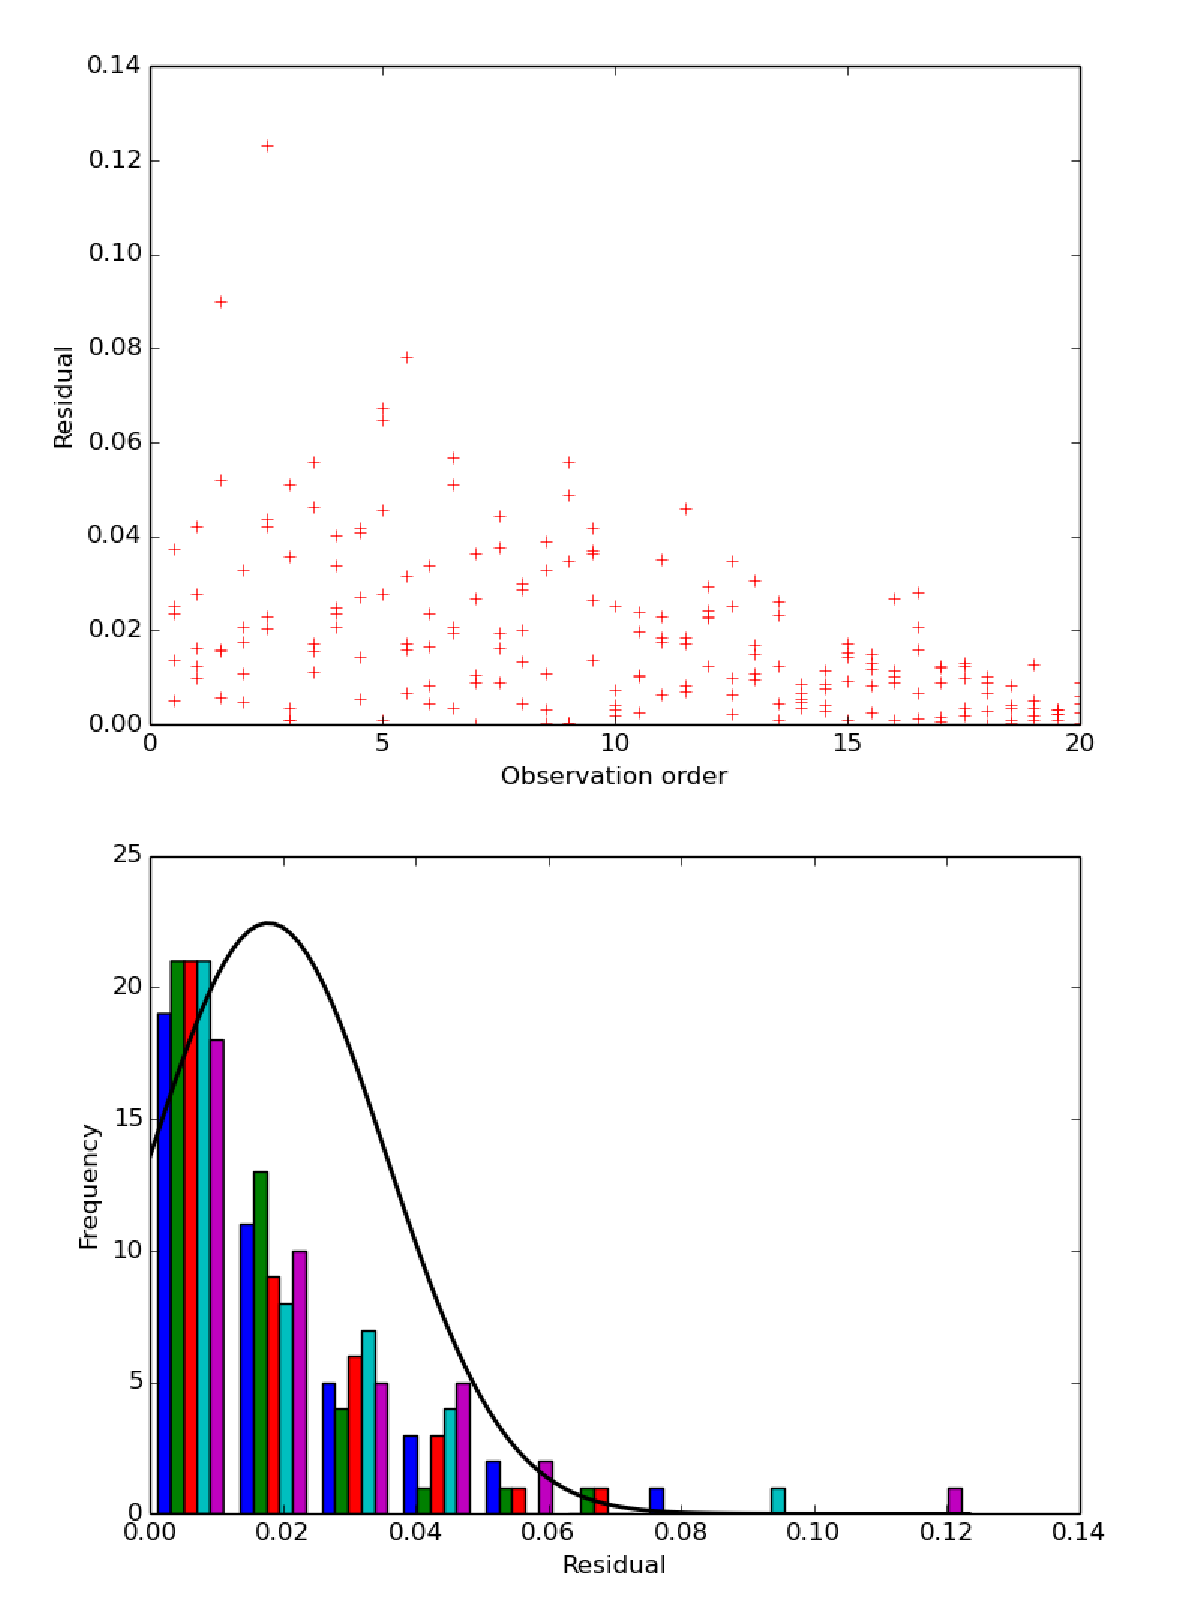
\includegraphics[width=\textwidth]{analysis_of_the_residuals.pdf}\\(a)
\end{minipage}\hfill
\begin{minipage}[c]{0.41\textwidth}
\centering
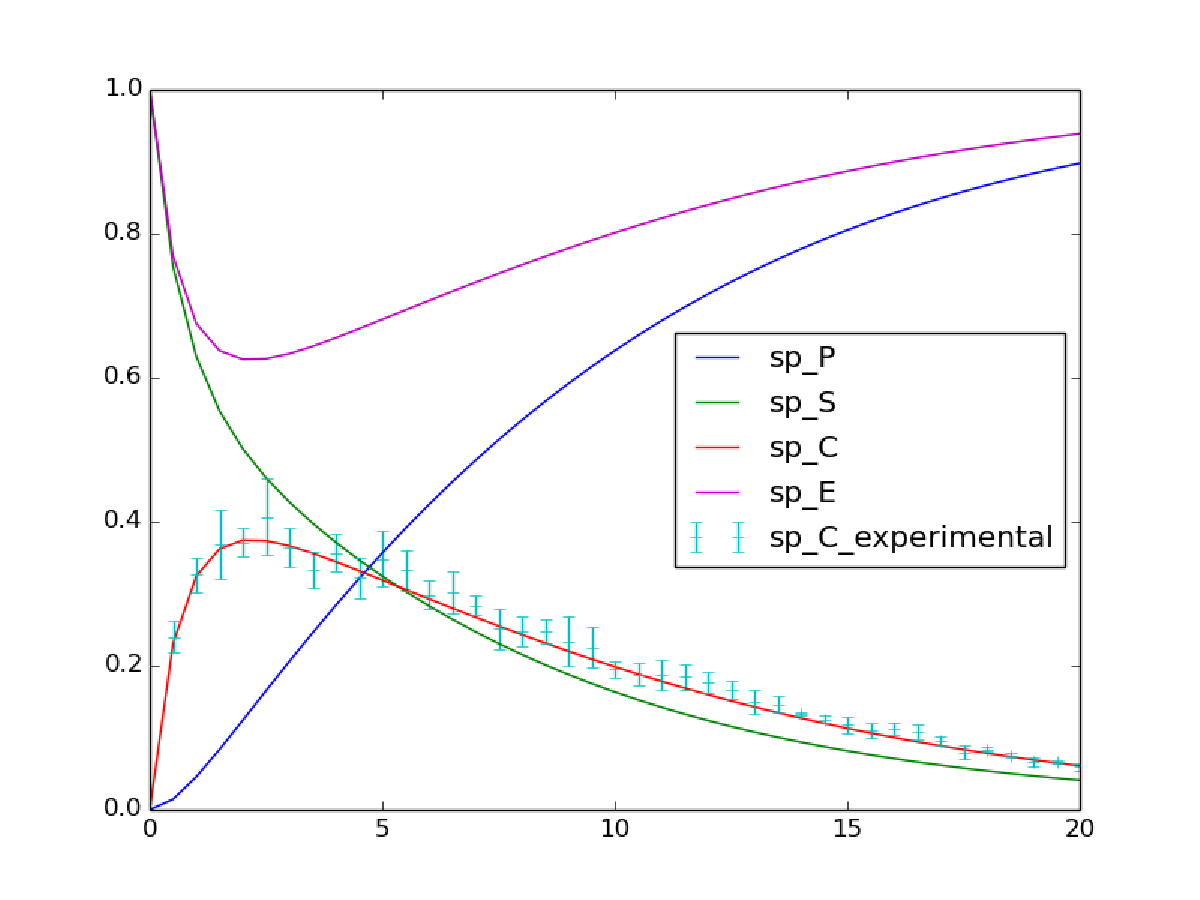
\includegraphics[width=\textwidth]{fitted_model.pdf}\\
(b)\\
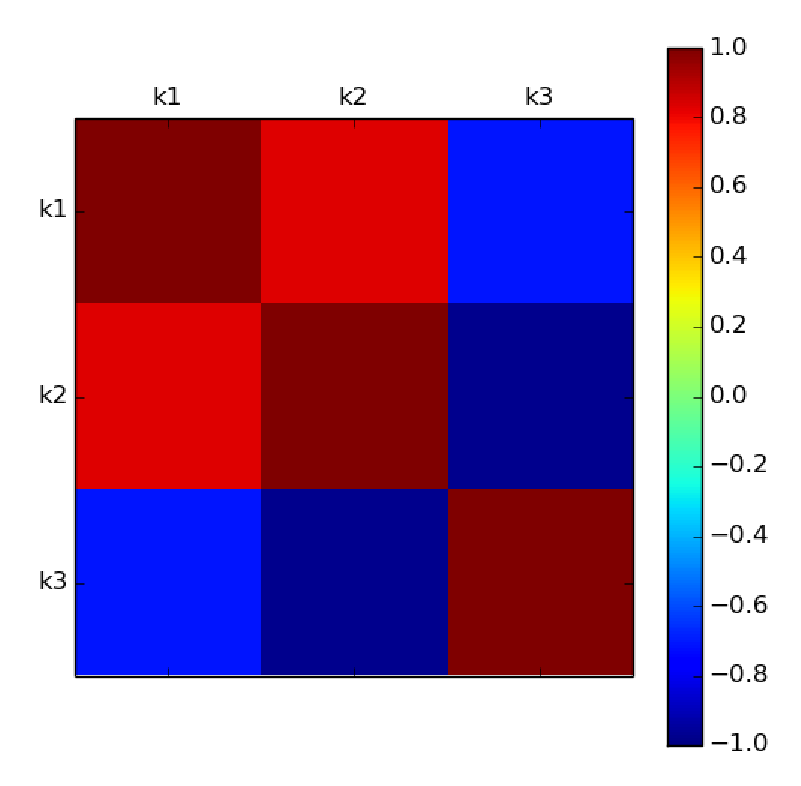
\includegraphics[width=\textwidth]{correlation_matrix.pdf}\\
(c)\\
\end{minipage}
\caption{Results of the parameter estimation described in Listing 2 using
the matplotlib library: (a) residual plot and frequency analysis of the
residuals; (b) simulated concentrations of species E, S, C and P versus time
using fitted parameters; (c) correlation matrix for the estimated parameters
$k_{1}$, $k_{2}$ and $k_{3}$.}
\end{center}
\end{figure}

\section{Conclusion}
The presented framework provides a {\bf high-level Python API} for executing
and manipulating analysis workflows written in SED-ML; simple workflows can be
directly executed while more elaborated ones can be scripted in Python. It
includes {\bf several simulation engines} dedicated to specific steps of the
{\bf systems biology model building cycle} and offers tools for {\bf exporting
and displaying numerical results}. The source code of the BioPreDyn software has
been {\bf released under the terms of the BSD 3-clause} open-source license and
is available on GitHub at {\bf https://github.com/TheCoSMoCompany/biopredyn}.
\bibliography{references}{}
\bibliographystyle{plain}
\end{multicols}
\end{document}
